\documentclass[12pt, a4paper, titilepage]{article}
\usepackage{graphicx}
\usepackage{subcaption}
\graphicspath{{C:/Users/huawei/Desktop/images/}} 
\usepackage{setspace}
\usepackage[english]{babel}
\usepackage[utf8x]{inputenc}
\usepackage{amsmath}
\usepackage{hyperref}
\usepackage{apacite}
\usepackage{titlesec}
\usepackage{dcolumn}
\usepackage{lscape}
\usepackage{pdflscape}
\usepackage{tabularx}
\usepackage{xcolor}
\usepackage{multirow}
\usepackage{times}
\usepackage{booktabs}
\usepackage{fancyhdr}
\usepackage[margin=1in]{geometry}
\usepackage{color}
\usepackage{dcolumn}
\usepackage{siunitx}
\usepackage{array}
\usepackage{longtable}
\usepackage{lineno}
\usepackage{array}
\usepackage{siunitx}
\usepackage{listings}
\usepackage{regexpatch}
\usepackage{multicol}
\usepackage{bm}
\usepackage{easyReview}
\usepackage{color, colortbl} %righe colorate
%opening
\DeclareMathOperator*{\argmax}{arg\,max}
\DeclareMathOperator*{\argmin}{arg\,min}
\title{It's how you use the items that counts: \\ An intelligent procedure for item selection in Item Response Theory}
\author{Ottavia M. Epifania\textsuperscript{1,2}, Pasquale Anselmi\textsuperscript{2}, \& Egidio Robusto\textsuperscript{2}}
\date{\textsuperscript{1}Department of Psychology and Cognitive Sciences, University of Trento \newline \textsuperscript{2}Department of Philosophy, Sociology, Education and Applied Psychology, University of Padova}

\begin{document}

\onehalfspacing

\maketitle

\begin{abstract}
Item Response Theory (IRT) provides the ideal framework for generating short test forms (STFs) from item banks or full-length tests. The usual procedure for developing STFs is based on the visual inspection of the item and test information functions (IIFs and TIFs) to find the items that best contribute to make up a STF with the desired characteristics. This contribution presents a new procedure that aims at automating this process by defining a target TIF and finding the items from the item bank that best recover it. The algorithm directly compares the distance between the target TIF and a temporary TIF obtained by adding an item at a time. The items are chosen according to their closeness to the location on the latent trait where the distance between the target and temporary TIFs is maximum. The algorithm stops when the addition of a new item does not reduce the distance between target and temporary TIFs. The procedure can be applied both when the length of the STF is defined a priori and the optimal number of items has to be find. The results of the application of this procedure are presented. 

\noindent \textbf{Keywords}:  Item Response Theory, Test Information Function, short test forms, intelligent search algorithm 
\end{abstract}

\newpage

\section*{Introduction}

Item Response Theory (IRT) models allow for estimating the probability that each person will endorse an item given their latent trait level and the characteristics of the items, as described by different parameters. The details at the item level inform about the precision with which each item measures different levels of the latent trait. As such, IRT models are of great use for developing short test forms (STFs), given the possibility they provide of minimizing the number of administered items while maximizing measurement precision.

Different procedures for the development of STFs based on IRT models exist, which are aimed at either the adaptive selection of items (i.e., each person is administered a different subset of items tailored to their specific latent trait level) or the fixed selection of items (i.e., static STFs where all people are administered the same subset of items). This contribution focuses on the development of static STFs. As such, if not otherwise specified, STFs identifies static STFs.
Recently, \citeA{pauci} introduced a new procedure for the development of STFs. This procedure is based on the a priori definition of the so-called $\theta$ targets, which are the levels of the latent trait on which the measurement precision should be focused the most. Although the procedure proved its soundness in developing STFs able to precisely measure the entire latent trait, the number of items to include in the STFs must be known in advance (it actually equals the number of $\theta$ targets).

In this contribution, a new procedure is introduced, which aims at developing STFs with characteristics that match those of a theoretically defined information function describing the characteristics of the desired test. As such, the number of items does not need to be set in advance. The procedure is validated through simulation studies and its performance is compared against a “brute force” procedure. The manuscript is organized as follows: the following section presents the 2-Parameter logistic model \cite<2-PL,>{birnbaum1968} and the information functions of the items and of the test. The descriptions of the newly introduced procedure and of the brute force procedure follow. Then, the simulation study is presented along with its results. A brief section illustrating the potentials and pitfalls of this procedure concludes the argumentation.
%This procedure is based on the automation of what is typically done in IRT for developing STF, that is trying to match a theoretically defined information function by including the items whose information functions best 

%Breve (Ottavia breve è chiaro?) sulle procedure per sviluppo della forma breve. 
%
%Citare il lavoro presentato a IMPS $\rightarrow$ molto figo ma devi sapere il numero di item in anticipo 
%
%Questa procedura non richiede di sapere il numero di item a priori ma scegie la combinazione di item migliore che si avvicini (i.e., che minimizzi la distanza da una test information function target). 
%
%Questo studio presenta un tentativo di validazione di questa procedura su dati simulati. la perfomance di questa procedura è confrontata con quella di una procedura (che viene chiamata forza bruta) dove vengono provate tutte le possibili combinazioni senza ripetizione degli item della item bank per trovare la forma breve di item che si avvicini il più possibile alla tif target. 


\subsection*{Item and Test Information Function in Item Response Theory}

Different IRT models are available according to the nature  of the observed responses (i.e., dichotomous vs. polytomous) and to the level of granularity desired for describing the functioning of the items (i.e., the number of item parameters). In this application, we refer to the 2-PL model \cite{birnbaum1968} for dichotomous responses. According to the 2-PL model, the probability of observing a correct response on item $i$ ($i = {1, 2, \ldots N}$) provided by person $p$ ($p = {1, 2, \ldots, P}$) is 

\begin{equation*}
	P(x_{pi} = 1|\theta_p, b_i, a_i) = \dfrac{\exp[a_i (\theta_p - b_i)]}{1 + \exp[a_i (\theta_p - b_i)]}, 
\end{equation*}
where $\theta_p$ describes the latent trait level of person $p$ (also known as ability parameter), $b_i$ is the difficulty of item $i$ (i.e., the location of the item on the latent trait), and $a_i$ is the discrimination parameter of item $i$, which describes the ability of the item to discriminate between respondents with different $\theta$ levels. 
The probability of a correct response depends on the distance on the latent trait between the person parameter $\theta_p$ and the item location $b_i$, such that if $\theta_p > b_i$ this probability is greater than $.50$, while if $\theta_p < b_i$ the same probability is lower than $.50$. This probability is further influenced by the discrimination parameter, such that the higher the value of $a_i$, the more two respondents with similar $\theta$ levels have different probabilities of endorsing the item. 
 
%The information each item provides with respect to each level of the latent trait $\theta$ is expressed via the \emph{item information function} (\emph{IIF}), $\mathit{IIF}_i= a_i^2[P(\theta, b_i, a_i)(1-P(\theta, b_i, a_i))].$
The \emph{item information function} (\emph{IIF}), $\mathit{IIF}_i= a_i^2[P(\theta, b_i, a_i)(1-P(\theta, b_i, a_i))]$, expresses the precision with which each item measures each level of the latent trait $\theta$.
%The IIF can be understood as the precision with which each item measures the levels of the latent trait. 
In the 2-PL model, the \emph{IIF} is strongly influenced by the discrimination parameter (i.e., the higher the value $a_i$ of item $i$, the higher its IIF) and it reaches its maximum (i.e., the item is mostly precise) when the ability $\theta_p$ matches the location $b_i$ of item $i$, such that $ P(\theta, b_i, a_i) = 1-P(\theta, b_i, a_i)$. 

By summing up the IIF of all the items, the \emph{test information function} (\emph{TIF}),  $\mathit{TIF} = \sum_{i = 1}^{N} IIF_i$, is obtained, which expresses the measurement precision of the test as a whole. Being the sum of IIFs, the TIF strongly depends on the number of items included in a test, and it can be increased just by adding new items. 
Given that the aim of the procedure introduced in this study is to minimize the number of administered items while recovering as best as possible the characteristics of a specific test, the use of the TIF as a criterion for choosing the most informative STF is misleading and would risk to favor STFs with a higher number of items.  
%Given the aim of this study (i.e., find an algorithm that minimizes the number of administered items while maximizing the precision of the assessment without relying on CAT procedures), 
%Given the aim of this study (i.e., find an algorithm that minimizes the number of administered items while maximizing the precision of the assessment without relying on CAT procedures), the use of the TIF as a criterion for choosing the most informative STF is misleading and would always favor STFs with a higher number of items. 
As such, the mean TIF, $\overline{\mathit{TIF}} = \sum_{i = 1}^{N} \frac{IIF_i}{N}$, is used as  criterion for choosing the most appropriate STF.
The logic underling $\overline{\mathit{TIF}}$ is that the higher the number of items included in the test, the higher the penalization of the TIF. In other words, for each $\theta$ level and given the same IIFs, STFs composed of fewer items would be favored. 

\section*{Item Selection Procedures}


This section presents two item selection procedures: (i) the \emph{item locating algorithm} (ILA), which is the procedure aimed at recovering a specific TIF determined a priori by locating the most appropriate items from the item bank, and (ii) the \emph{brute force procedure} (BFP), which selects the STF that best recovers the TIF determined a priori after trying all the possible combinations of items of different lengths. 

Both ILA and BFP require the definition of a TIF target, which describes the desired characteristics of the STF, regardless of its length. Both procedures attempt at recovering as best as they can the TIF target, denoted as $\mathit{TIF}^*$.
The BFP was introduced to check whether ILA is able to recover the best possible combination of items among all the possible combinations of items of different lengths that can be obtained from the item bank. The simulation study compares the performance of ILA and that of BFP in 100 simulations. Further details are provided in Section ``Simulation Study''.

\subsection*{Item Locating Algorithm}

%The item locating algorithm (ILA) is an iterative algorithm that requires the definition of a TIF target as starting point, denoted as $\mathit{TIF}^*$. 
%The TIF target defines the regions on the latent trait for which the STF should provide the highest information. The TIF target can be defined considering previous knowledge on the construct of interest. 
ILA is an iterative algorithm that compares the $\mathit{TIF}^*$ with temporary TIFs, denoted as $\mathit{TIF}_{TE}$, obtained at each iteration by adding one item at the time. ILA iterates until  the absolute difference between $\mathit{TIF}^*$ and the $\mathit{TIF}_{TE}$ that includes the last selected item is equal to or greater than the difference between the $\mathit{TIF}^*$ and the $\mathit{TIF}_{TE}$ that does not include the last selected item (i.e., termination criterion). Notably, $\mathit{TIF}_{TE}$  is the mean temporary TIF obtained as $TIF_{TE} = \frac{\sum_{i\in Q} IIF_i}{||Q||}$, where $||Q||$ denotes the cardinality of the vector $Q$ that contains the indexes of the items selected for inclusion in the STF up to that iteration. 

%that is obtained by averaging the TIF by the cardinality of $Q$ ($||Q||$), where 
%Deve avere diversi livelli di theta e per ognuno di essi un livello di informatività definito a livello teorico, empirico o tramite simulazioni. La TIF target viene definita da qui in avanti come $\mathit{TIF}^*$. 


%$\mathit{TIF}^*$: TIF Target

%$TIF_{TE} = \frac{\sum_{i\in Q} IIF_i}{||Q||}$, where $||X||$ identifies the cardinality of $X$

%$Q$: Set degli indici degli item selezionati per inclusione all'iterazione $k$. All'iterazione 1 (inizio dell'algoritmo, va deciso se far partire le iterazioni da 0 o da 1) $Q = \{\emptyset\}$

%\alert{Iterazioni $k = \{1, \ldots K\}$ $K$ è il momento in cui la differenza tra $TIF^*$ e $TIF_{TE}$ all'iterazione $k$ è uguale o maggiore della stessa differenza all'iterazione $k-1$.}

The algorithm iterates the following steps until the termination criterion is reached: 

\begin{enumerate}
\item  The absolute difference between $\mathit{TIF}^*$ and $TIF_{TE}$ is computed, $\Delta_{TIF} = |TIF^* - TIF_{\text{TE}}|$. Since at the beginning no items are selected for inclusion in the STF, $Q = \emptyset$ and $||Q|| =0$, so $\Delta_{TIF} = |TIF^* - 0|$. 
	
\item  A $\theta_{target}$ is determined as the $\theta$ level for which the absolute distance between the $\mathit{TIF}^*$ and $\mathit{TIF}_{TE}$ is maximum, $\argmax{\Delta_{TIF}}$. %At the first iteration, it will be the $\theta$ level with the highest information function. 
	
\item  The index of the first item to be included in $Q$ is the index of the item whose location is closest to the $\theta_{target}$, $\text{argmin}_{i \in \{1, \ldots, N\}\setminus Q} |\theta_{target} -b_i|$.
	
\item  The mean temporary TIF is computed as $TIF_{TE} = \frac{\sum_{i\in Q} IIF_i}{||Q||}$
	
\item  Repeat from Step 1 until the termination criterion is reached.
\end{enumerate}


%The first step of the algorithm is to find the $\theta$ level at iteration $k = 1$ where $\argmax{\mathit{TIF}^*}$. This $\theta$ level is denoted as $\theta_{target}$. 
%The index of the first item to be included in $Q$ is the item whose location is closest to the $\theta_{target}$, $\text{argmin}_{i \in \{1, \ldots, N\}\setminus Q} |\theta_{target} -b_i|$. Once the item is found, the mean temporary TIF is computed as $TIF_{TE} = \frac{\sum_{i\in Q} IIF_i}{||Q||}$, where $||X||$ identifies the cardinality of $X$.  

%The second step is to compute the absolute difference between the TIF tagret and the temp TIF, vector $\Delta_{TIF} = |TIF^* - TIF_{\text{TE}_k}|$. Then, the new theta target is the theta level that corresponds to the maximum value within vector $\Delta_{TIF}$, $\argmax{\Delta_{TIF}}$. Once the $\theta_{target}$ is identified, the procedure starts again searching for the items in $N\setminus Q$ the items whose location is the closest to the identified $\theta_{target}$

%
%\alert{The procedure iterates until the termination criterion is reached, that is when the absolute difference between the tif target and the temporary tif at iteration k is greater or equal to the difference between the same two quantities at iteration $k-1$.
%	$\Delta_{TIF} = |TIF^* - TIF_{\text{TE}_k}| \geq \Delta_{TIF} = |TIF^* - TIF_{\text{TE}_{k-1}}|$ 
%}

%The first step of the algorithm is to find the $\theta$ level for which $\max{\mathit{TIF}^*}$, denoted as $\theta_{target}$. 
%Let $Q$ be the set of indexes identifying the items selected at each iteration to be included in the STF. At the beginning of the algorithm $Q = \{\emptyset\}$. The first item to be included in $Q$ is the item whose location is the closest to  $\theta_{target}$ credo che sia $\text{argmin}_{i \in \{1, \ldots, N\}\setminus Q} |\theta_{target} -b_i|$



%
%The next step of the che cazzo poi lo trovo è $\max{\Delta_{TIF}}$ trova il thet atrget per il max delta tif 
%
%
%Definisco un vettore $Q$ degli item che vengono inclusi a ogni iterazione. Il numero di iterazioni non è definito a priori. 
%
%Si definisce una TIF target (che penso sia una TIF target media)
%
%Il primo item viene scelto come l'item con la location o la IIF maggiore in prossimità del theta per cui la TIF è massima. 
%
%L'item viene messo dentro il test, si calcola la TIF media e si calcola la differenza assoluta tra la tif media target e la tif temporanea. 
%L'item inserito è quello con la location più vicina al theta per cui la differenza assoluta è massima (oppure l'item con la IIF più alta with respect to the theta where the diference between the TIF target and the temporary TIF is maximed). 
%
%The procedure goes on and on and on untile the additon of an item to the temporary tif does not produce an improvement in the temporary tif (i.e., the absolute difference does not change).

\section*{The Brute Force Procedure}

%The performance of the Ilocate algorithm in selecting the items for producing a test able to minimize the distance from a TIF target has been compared to an item selection based on the ``brute force''. 
BFP develops the STFs considering all the possible  combinations of items without repetition and compares the STFs from those of length 1 (i.e., those composed of one item only) to those of length $L$, where $L = N- 1$ and $N$ is the number of items included in the item bank. For each of the possible lengths $l = \{1, \ldots L\}$ of the STF, a $\binom{N}{l}$ number of STFs is developed. 
For instance, if the item bank is composed of $N = 10$ items, $l = \{1, \ldots, 9\}$, and the BFP will develop $\binom{10}{1} + \binom{10}{2} + \binom{10}{3} + \binom{10}{4} + \binom{10}{5} + \binom{10}{6} + \binom{10}{7} + \binom{10}{8} + \binom{10}{9} = 1,022$ STFs. 

For each of the possible combinations of items of length $l$,  the $\overline{\mathit{TIF}}$ is computed, and the absolute difference from the TIF target, $\Delta_{TIF} = TIF^* - \overline{\mathit{TIF}}$, and a mean of the absolute difference are obtained $\overline{\Delta}_{TIF}$.
The best STF is the one with the lowest value of $\overline{\Delta}_{TIF}$, that is the one that presents the lowest absolute distance from the TIF target.


\section*{Simulation Study}
The simulation study was run in \texttt{R} \cite{rsoft}, and it iterated the following steps for 100 times: 

\begin{enumerate}
	\item  Generate an item bank composed of $N = 6$ items with difficulty parameters drawn from a uniform distribution $\mathcal{U}(-3, 3)$ and discrimination parameters drawn from a uniform distribution $\mathcal{U}(.90, 2.0)$;
	
	\item  Generate a mean TIF target by randomly selecting items from the item bank. The number of selected items varied between 2 and 5 (Mean $= 3.34 \pm 1.13$).
	The starting difficulty and discrimination parameters of the selected items are modified by adding or subtracting values randomly extracted, at each iteration, from uniform distributions $\mathcal{U}(-0.20, 0.20)$. A constraint is made on the discrimination parameters such that they cannot result in negative values after they are modified through the addition or subtraction of the value;
	
	
	\item  Considering the TIF defined at Step 2 and the item parameters generated at Step 1:
	\begin{itemize}
		\item ILA searches for the best possible STF able to recover the TIF target
		\item BFP looks for the best possible item combination. Given that the item bank is composed of $N=6$ items, $L = 5$ and $\binom{6}{1} + \binom{6}{2} + \binom{6}{3} + \binom{6}{4} + \binom{6}{5} =  62$ STFs are developed and compared.
	\end{itemize}
	
\end{enumerate}

To evaluate the performance of ILA, the following criteria have been followed: 

\begin{itemize}
	\item  Symmetric distance between the indexes of the items selected by BFP and ILA. On the ground of the symmetric distance, it is possible to compute the sensitivity (i.e., the number of items that are identified by BFP and selected by ILA), specificity (i.e., the number of items that have been excluded by both BFP and ILA), and accuracy (the sum between specificity and sensitivity divided by the length of the item bank).
	
	\item  Rank of the STF obtained with ILA in the distribution of STFs obtained with BFP, ordered according to their increasing distance from the average TIF of the STFs that best resemble the TIF target. 
	
\end{itemize}


Moreover, the occurrences in which the cardinalities of $Q$ were equal according to both ILA and BFP $||Q_{\text{ILA}}|| = ||Q_{\text{BFP}}||$ were counted in each iteration. 
If $||Q_{\text{ILA}}|| = ||Q_{\text{BFP}}||$, then we checked whether the two strategies resulted in the same selection of items. 
Otherwise, the difference between the cardinalities was computed as $||Q_{\text{ILA}}|| - ||Q_{\text{BFP}}||$ and it was averaged across the iterations. 

\section*{Results}

Among the 100 simulations, ILA and BFP resulted in STFs of same lengths in 57 cases, out of which 41 cases resulted in the same selection of items. In the 34\% of cases, ILA selected less items than BFP, while it selected more items than BFP in the 9\% of cases. The weighted mean of item difference between ILA and BFP was $0.77$. 

Averaging across the 100 iterations, ILA included the same items as BFP (sensitivity) and excluded the same items as BFP (specificity) in the 72\% and 85\% of the occurrences, respectively. 

Concerning the percentile rank of the distance from the best STFs identified by BFP, in the 74\% of instances ILA produced STFs within the 10nth percentile of distance, while the median percentile rank was $3.17$. This means that in the 50\% of the cases, ILA developed a STF that was within the fourth percentile of distance from the best possible STF. 

%\begin{figure}
%	\centering
%	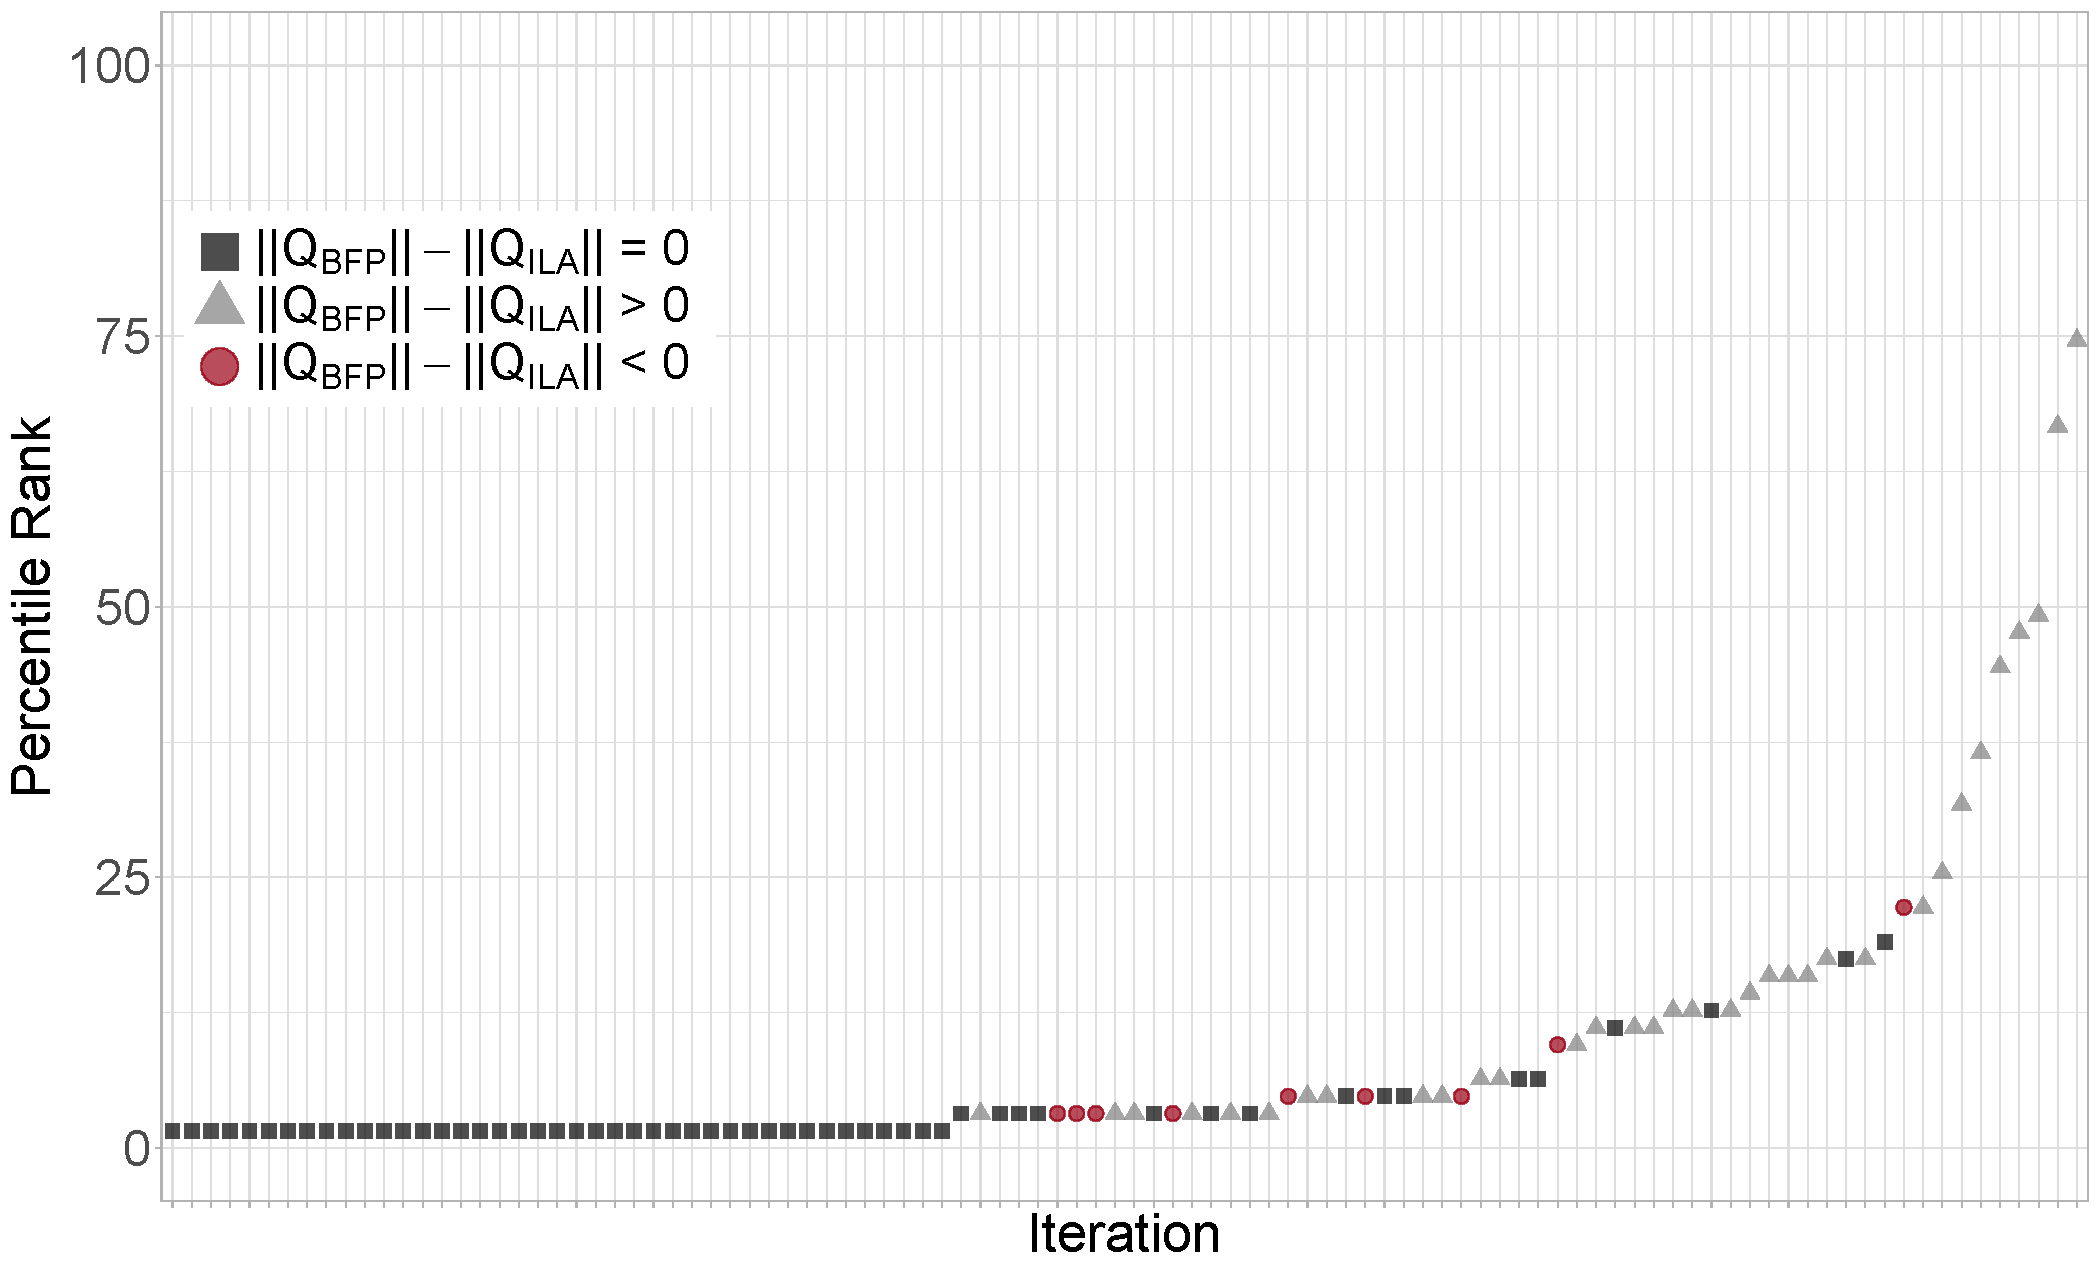
\includegraphics[width=\linewidth]{rp}
%\end{figure} 

\section*{Final Remarks}
As suggested by the results of the simulation study, ILA appears to be a promising algorithm for shortening tests in an IRT framework. Nonetheless, work is still needed. As it is now, ILA grounds item selection only on the item location with respect to the identified $\theta$ target. Future developments of the algorithm should consider the discrimination parameter as well, possibly by grounding the item selection on their information functions with respect to the $\theta$ target. 
 

\bibliographystyle{apacite} 
\bibliography{bibFile.bib}

\end{document}
